\chapter{Теоретический раздел}

DES (in English, Data Encryption Standard)~---~алгоритм для симметричного шифрования, разработанный фирмой IBM и утверждённый правительством США в 1977 году как официальный стандарт. Размер блока для DES равен 64 битам. В основе алгоритма лежит сеть Фейстеля с 16 циклами (раундами) и ключом, имеющим длину 56 бит. Алгоритм использует комбинацию нелинейных ($S$-блоки) и линейных (перестановки $E$, $IP$, $IP^{-1}$) преобразований. Для DES рекомендовано несколько режимов:

\begin{itemize}
	\item ECB (electronic code book)~---~режим «электронной кодовой книги» (простая замена);
	\item CBC (cipher block chaining)~---~режим сцепления блоков;
	\item PCBC (propagating cipher block chaining)~---~режим распространяющегося сцепления блоков;
	\item CFB (cipher feed back)~---~режим обратной связи по шифротексту;
	\item OFB (output feed back)~---~режим обратной связи по выходу;
	\item Counter Mode (CM)~---~режим счётчика.
\end{itemize}
     
Прямым развитием DES в настоящее время является алгоритм Triple DES (3DES). В 3DES шифрование/расшифровка выполняются путём троекратного выполнения алгоритма DES. 

\section{Описание алгоритма DES}

На рисунке \ref{fig:des_basic_schema} представлена базовая схема работы алгоритма DES.

\newpage

\begin{figure}[h!]
\centering
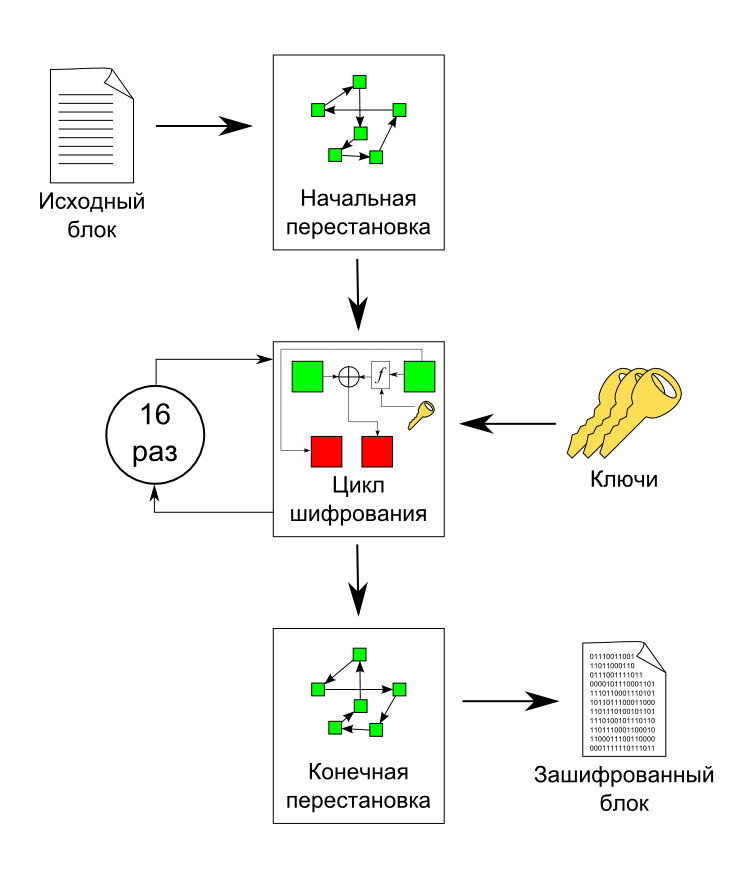
\includegraphics[width=0.5\textwidth]{assets/des_basic_schema.png}
\caption{Базовая схема работы алгоритма DES}
\label{fig:des_basic_schema}
\end{figure}

Выполнение алгоритма можно разделить на несколько этапов. Расшифровка представляет собой повторение действий шифрования в обратном порядке. Более подробная схема алгоритма DES представлена на рисунке \ref{fig:des_1}.

\newpage

\begin{figure}[h!]
\centering
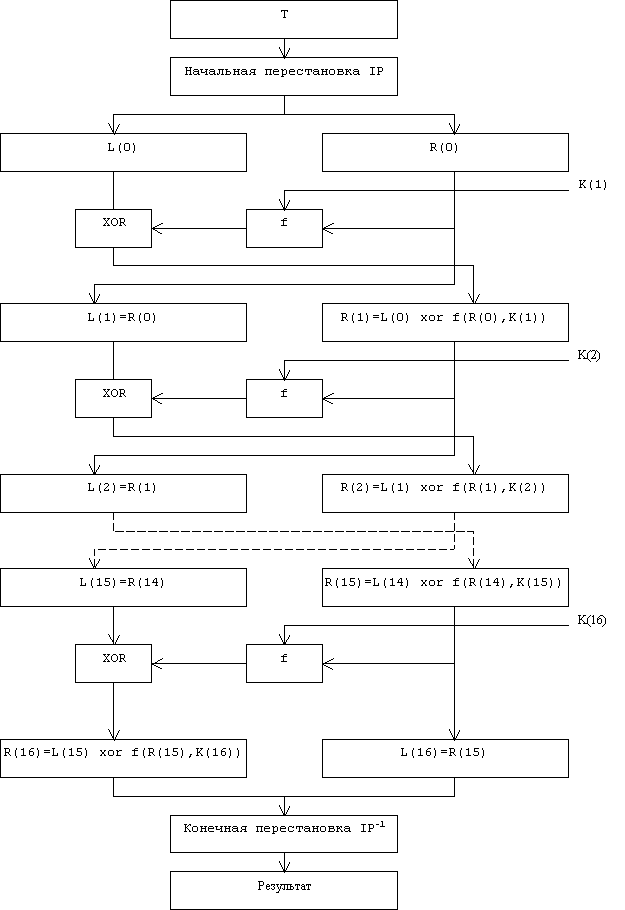
\includegraphics[width=0.5\textwidth]{assets/des.png}
\caption{Подробная схема работы алгоритма DES}
\label{fig:des_1}
\end{figure}

\subsection{Начальная перестановка}

Исходный текст $T$ преобразуется с помощью таблицы $IP$. Преобразование выполняется по следующему принципу: первый бит результата будет равен значению бита $T$ с номером, равным значению в таблице.

\begin{center}
\begin{tabular}{|r|r|r|r|r|r|r|r|r|r|r|r|r|r|r|r|} 
 \hline
58 & 50 & 42 & 34 & 26 & 18 & 10 & 2 & 60 & 52 & 44 & 36 & 28 & 20 & 12 & 4 \\ 
\hline
62 & 54 & 46 & 38 & 30 & 22 & 14 & 6 & 64 & 56 & 48 & 40 & 32 & 24 & 16 & 8 \\ 
\hline
57 & 49 & 41 & 33 & 25 & 17 & 9 & 1 & 59 & 51 & 43 & 35 & 27 & 19 & 11 & 3 \\ 
\hline
61 & 53 & 45 & 37 & 29 & 21 & 13 & 5 & 63 & 55 & 47 & 39 & 31 & 23 & 15 & 7 \\ 
\hline
\end{tabular}
\end{center}

\subsection{Циклы шифрования}

После начальной перестановки блок $IP(T)$ участвует в 16 циклах преобразования Фейстеля. Сначала блок разбивается на два 32-битных блока $L_0$ и $R_0$ ($R_0$~---~младшая половина).

Тогда в течение 16 итерации можно использовать следующие соотношения:

\begin{equation*}
	L_i = R_{i-1}
\end{equation*}

\begin{equation*}
	R_i = L_{i-1} \oplus f(R_{i-1}, k_i)
\end{equation*}


\subsubsection{Функция Фейстеля}

$f(R_{i-1}, k_i)$~---~функция Фейстеля. Для вычисления нужно выполнить следующие шаги.

Во-первых, использовать на аргументе ($R_{i-1}$) функцию расширения $E$, заданную таблицей. Функция позволяет расширить 32-битный аргумент до 48 бит.

\begin{center}
\begin{tabular}{|r|r|r|r|r|r|} 
 \hline
32 & 1 & 2 & 3 & 4 & 5 \\ \hline
4 & 5 & 6 & 7 & 8 & 9 \\ \hline
8 & 9 & 10 & 11 & 12 & 13 \\ \hline
12 & 13 & 14 & 15 & 16 & 17 \\ \hline
16 & 17 & 18 & 19 & 20 & 21 \\ \hline
20 & 21 & 22 & 23 & 24 & 25 \\ \hline
24 & 25 & 26 & 27 & 28 & 29 \\ \hline
28 & 29 & 30 & 31 & 32 & 1 \\ \hline
\end{tabular}
\end{center}


Во-вторых, результат расширения сложить по модулю 2 с ключом $k_i$ и разбить на 8 блоков по 6 бит.

\begin{equation*}
	E(R_{i-1}) \oplus k_i = B_1B_2B_3B_4B_5B_6B_7B_8
\end{equation*}

В-третьих, каждый $i$-ый блок нужно преобразовать с помощью соответственной таблицы $S_i$. Пример таблицы $S_1$ приведен ниже. На основании крайних битов определется строка таблицы, на основании серединных четырех~---~столбец. На пересечении стоит четырехбитное число, которое и будет результатом преобразования.

\begin{center}
\begin{tabular}{|r|r|r|r|r|r|r|r|r|r|r|r|r|r|r|r|r|} 
 \hline
 & \textbf{0} & \textbf{1} & \textbf{2} & \textbf{3} & \textbf{4} & \textbf{5} & \textbf{6} & \textbf{7} & \textbf{8} & \textbf{9} & \textbf{10} & \textbf{11} & \textbf{12} & \textbf{13} & \textbf{14} & \textbf{15} \\ \hline
\textbf{0} & 14 & 4 & 13 & 1 & 2 & 15 & 11 & 8 & 3 & 10 & 6 & 12 & 5 & 9 & 0 & 7 \\ \hline
\textbf{1} & 0 & 15 & 7 & 4 & 14 & 2 & 13 & 1 & 10 & 6 & 12 & 11 & 9 & 5 & 3 & 8 \\ \hline
\textbf{2} & 4 & 1 & 14 & 8 & 13 & 6 & 2 & 11 & 15 & 12 & 9 & 7 & 3 & 10 & 5 & 0  \\ \hline
\textbf{3} & 15 & 12 & 8 & 2 & 4 & 9 & 1 & 7 & 5 & 11 & 3 & 14 & 10 & 0 & 6 & 13 \\ \hline
\end{tabular}
\end{center}

После преобразовании четырехбитные блоки склеиваются в один 32-битный, к этому блоку применяется перестановка $P$.

\begin{center}
\begin{tabular}{|r|r|r|r|r|r|r|r|} 
 \hline
16 & 7 & 20 & 21 & 29 & 12 & 28 & 17 \\ \hline
1 & 15 & 23 & 26 & 5 & 18 & 31 & 10 \\ \hline
2 & 8 & 24 & 14 & 32 & 27 & 3 & 9 \\ \hline
19 & 13 & 30 & 6 & 22 & 11 & 4 & 25 \\ \hline
\end{tabular}
\end{center}

Схема алгоритма функции Фейстеля представлена на рисунке \ref{fig:f}.

\begin{figure}[h!]
\centering
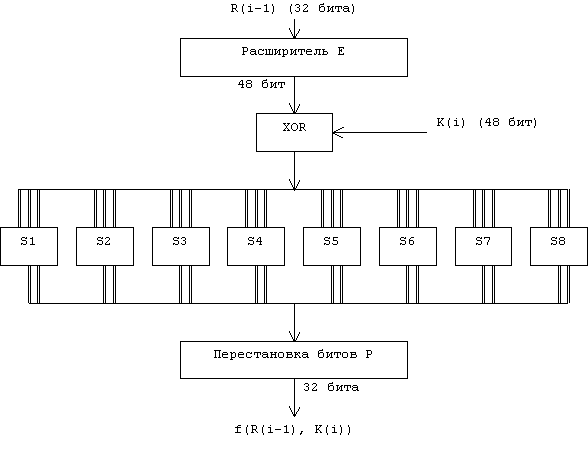
\includegraphics[width=0.65\textwidth]{assets/f.png}
\caption{Схема алгоритма функции Фейстеля}
\label{fig:f}
\end{figure}

\subsubsection{Генерация ключей}
Начальный ключ состоит из 64 бит. С помощью функции $G$ из него убираются контрольные биты и производится перестановка.

\begin{center}
\begin{tabular}{|r|r|r|r|r|r|r|r|r|r|r|r|r|r|} 
 \hline
57 & 49 & 41 & 33 & 25 & 17 & 9 & 1 & 58 & 50 & 42 & 34 & 26 & 18 \\ \hline
10 & 2 & 59 & 51 & 43 & 35 & 27 & 19 & 11 & 3 & 60 & 52 & 44 & 36 \\ \hline
63 & 55 & 47 & 39 & 31 & 23 & 15 & 7 & 62 & 54 & 46 & 38 & 30 & 22 \\ \hline
14 & 6 & 61 & 53 & 45 & 37 & 29 & 21 & 13 & 5 & 28 & 20 & 12 & 4 \\ \hline
\end{tabular}
\end{center}

Получившаяся в результате перестановки 56-битная последовательность разбивается на две половины~---~$C_0$ и $D_0$ ($D_0$~---~младшая).

Для $i$ от $1$ до $16$ с этими половинами производятся циклические сдвиги влево в соответствии с таблицей.

\begin{center}
\begin{tabular}{|l|r|r|r|r|r|r|r|r|r|r|r|r|r|r|r|r|r|} 
 \hline
i & 1 & 2 & 3 & 4 & 5 & 6 & 7 & 8 & 9 & 10 & 11 & 12 & 13 & 14 & 15 & 16 \\ \hline
shift & 1 & 1 & 2 & 2 & 2 & 2 & 2 & 2 & 1 & 2 & 2 & 2 & 2 & 2 & 2 & 1 \\ \hline
\end{tabular}
\end{center}

Получившиеся блоки склеиваются и производится перестановка в соответствии с таблицей. При этом, из 56-битного ключа, на каждой итерации получается 48-битный ключ.

\begin{center}
\begin{tabular}{|r|r|r|r|r|r|r|r|r|r|r|r|r|r|r|r|r|} 
 \hline
14 & 17 & 11 & 24 & 1 & 5 & 3 & 28 & 15 & 6 & 21 & 10 & 23 & 19 & 12 & 4 \\ \hline
26 & 8 & 16 & 7 & 27 & 20 & 13 & 2 & 41 & 52 & 31 & 37 & 47 & 55 & 30 & 40 \\ \hline
51 & 45 & 33 & 48 & 44 & 49 & 39 & 56 & 34 & 53 & 46 & 42 & 50 & 36 & 29 & 32  \\ \hline
\end{tabular}
\end{center}

\subsection{Конечная перестановка}

Блоки $L_{16}$ и $R_{16}$ объединяются в блок $T_{16}$ ($R_{16}$~---~старшая половина!). Блок $T_{16}$ преобразуется с помощью таблицы $IP^{-1}$. Преобразование выполняется по следующему принципу: первый бит результата будет равен значению бита $T$ с номером, равным значению в таблице.

\begin{center}
\begin{tabular}{|r|r|r|r|r|r|r|r|r|r|r|r|r|r|r|r|} 
 \hline
40 & 8 & 48 & 16 & 56 & 24 & 64 & 32 & 39 & 7 & 47 & 15 & 55 & 23 & 63 & 31 \\ \hline
38 & 6 & 46 & 14 & 54 & 22 & 62 & 30 & 37 & 5 & 45 & 13 & 53 & 21 & 61 & 29 \\ \hline
36 & 4 & 44 & 12 & 52 & 20 & 60 & 28 & 35 & 3 & 43 & 11 & 51 & 19 & 59 & 27 \\ \hline
34 & 2 & 42 & 10 & 50 & 18 & 58 & 26 & 33 & 1 & 41 & 9 & 49 & 17 & 57 & 25 \\ \hline
\end{tabular}
\end{center}

\section{Описание режима шифрования CBC}

В режиме сцепления блоков (CBC) каждый блок открытого текста складывается по модулю два с предыдущим блоком шифротекста, а затем шифруется. Таким образом, каждый блок шифротекста зависит от всех обработанных блоков открытого текста. Чтобы каждое сообщение было уникальным, при обработке первого блока открытого текста должна использоваться синхропосылка. Режим сцепления блоков является наиболее часто используемым.

На рисунках \ref{fig:cbc_encryption}~--~\ref{fig:cbc_decryption} представлена базовая схема работы режима шифрования и расшифрования CBC.

\begin{figure}[h!]
\centering
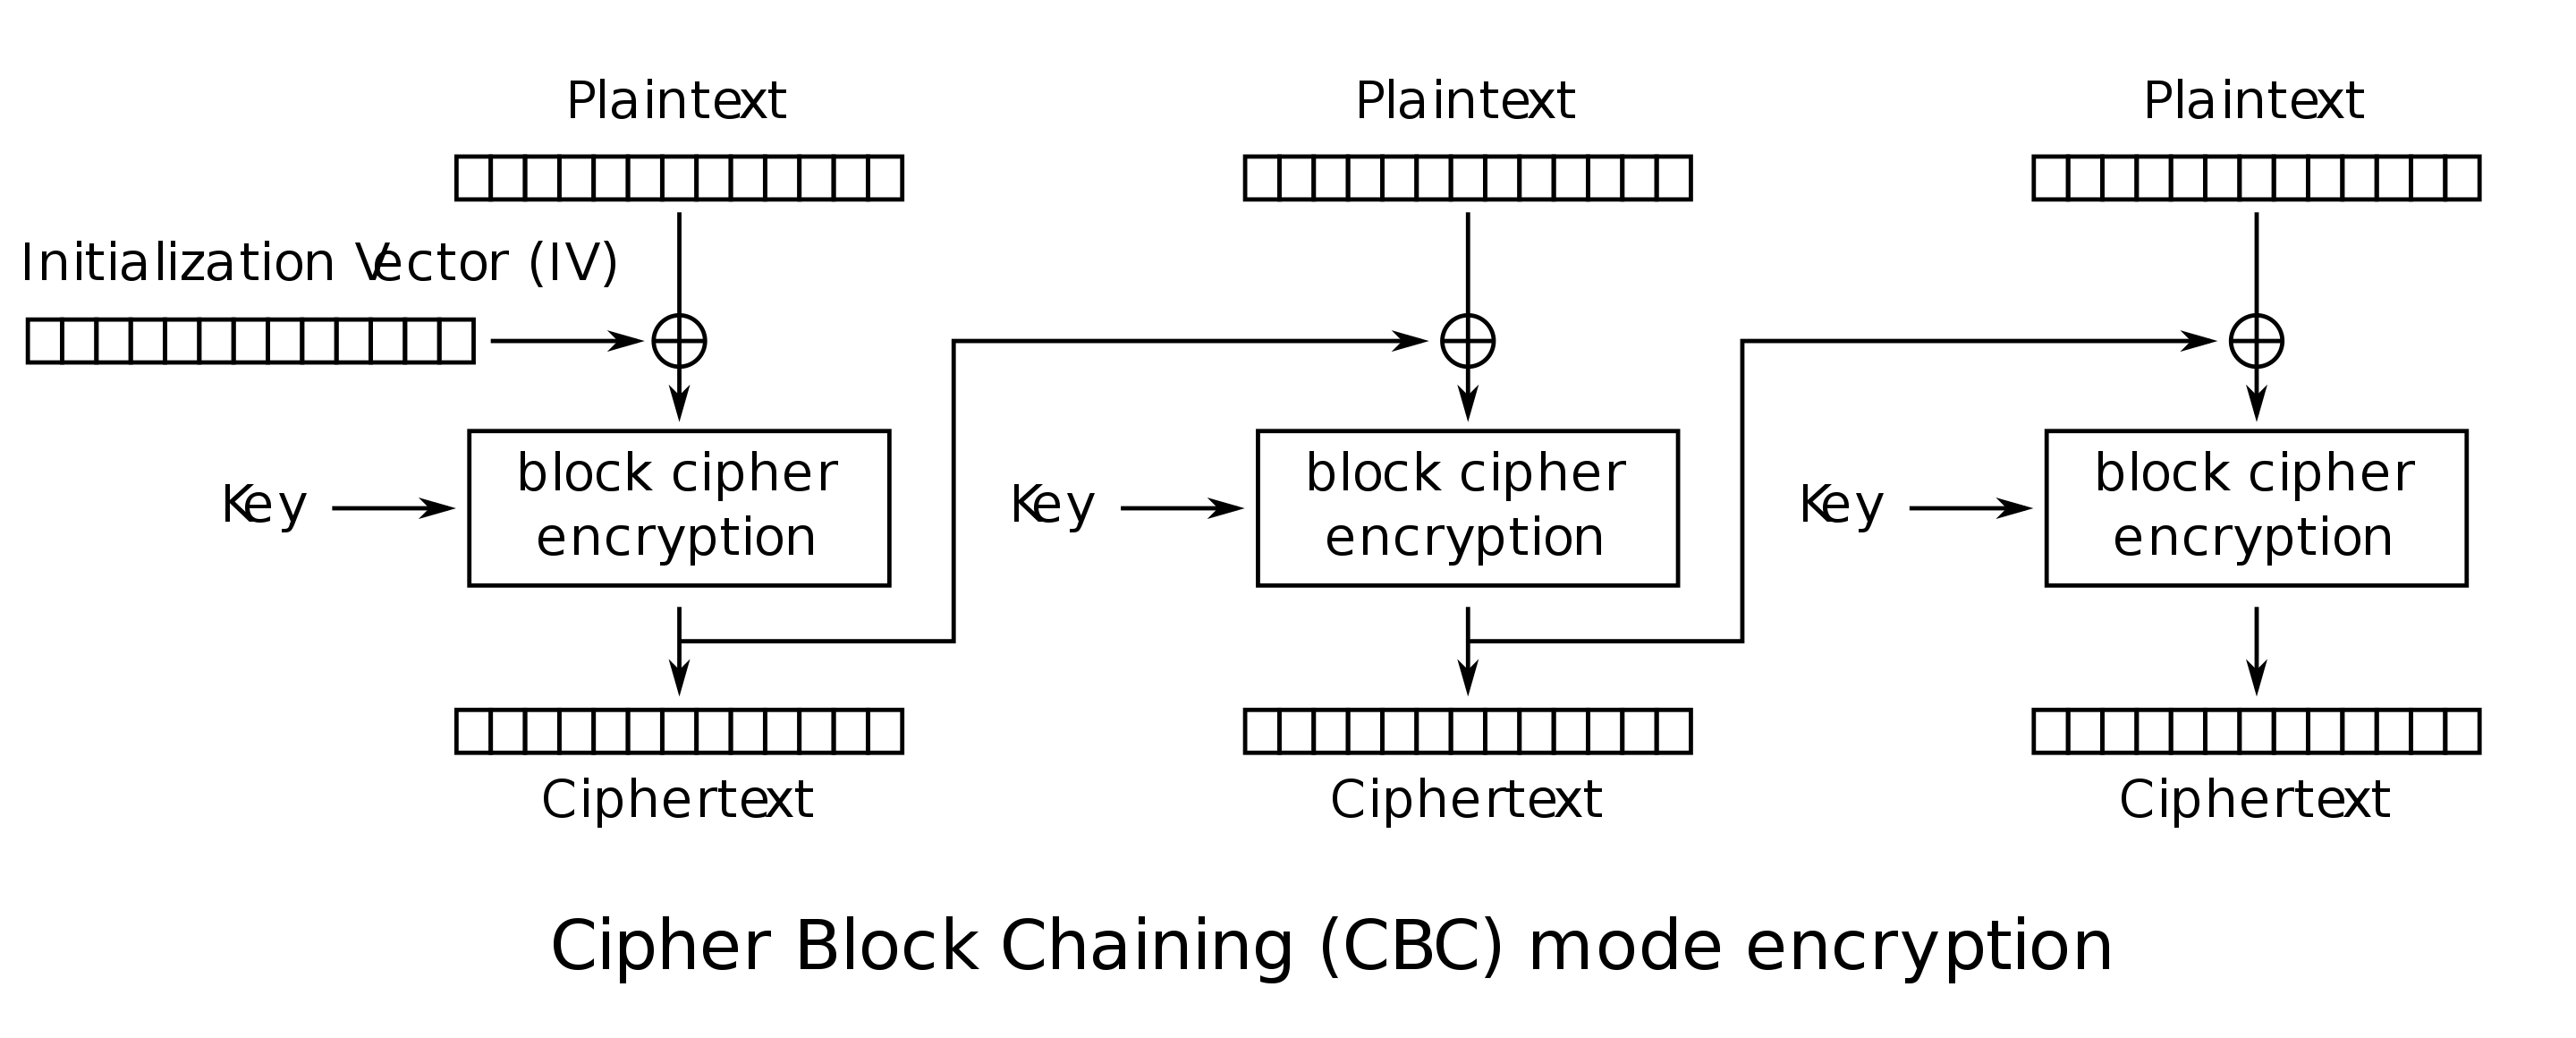
\includegraphics[width=0.75\textwidth]{assets/cbc_encryption.png}
\caption{Шифрование с использованием CBC}
\label{fig:cbc_encryption}
\end{figure}

\begin{figure}[h!]
\centering
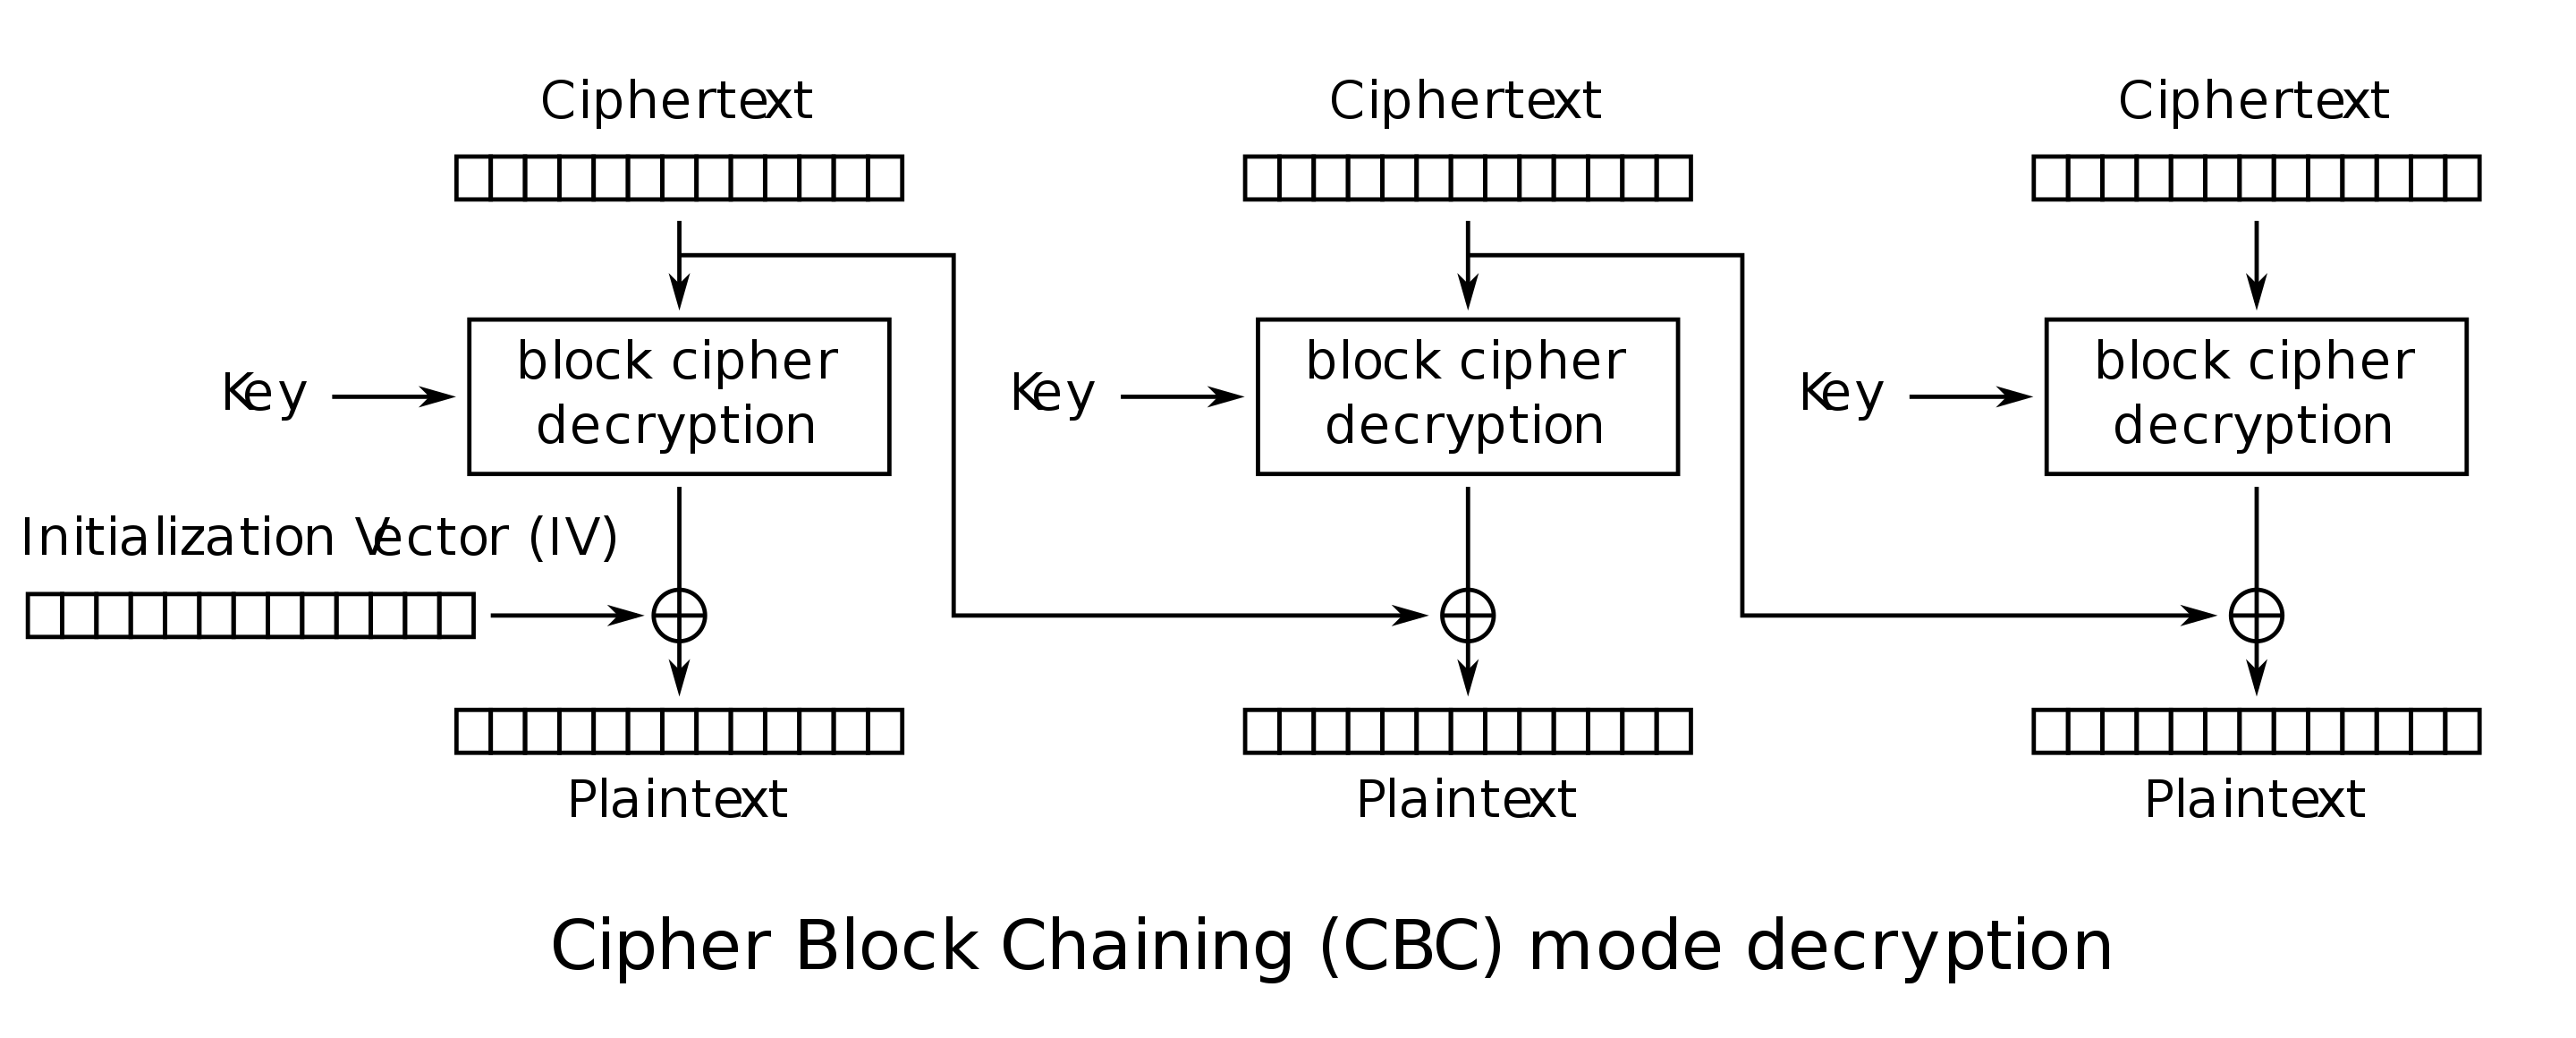
\includegraphics[width=0.75\textwidth]{assets/cbc_decryption.png}
\caption{Расшифровка с использованием CBC}
\label{fig:cbc_decryption}
\end{figure}
